%!TEX root = thesis.tex
\chapter{Model implementation}\label{chap:methods}
\thispagestyle{plain}

This chapter describes the model implementation process, including the underlying theory.
The first section explains the general concepts of the glacier volume/area scaling relation as well as the theoretical basis for the implemented temperature-index mass balance model and glacier evolution model. Programming related implementation details are shown in the second section, including the description of relevant classes and methods. This can be seen as a simple documentation. The third and final section of this chapter details the experimental setup for the following model evaluation.

% ==== SECTION 1 ===============================================================
\section{General concepts} % (fold)
\label{sec:general_concepts}

    Before starting to write any code, a solid theoretical foundation has to be established. A summary of the extensive work on \vas{} \citep{Bahr1997, Bahr1997a, Bahr1997b, Bahr2015} is provided,  including a discussion about the ill-posed nature of ice volume inversions \citep{Bahr2014}. The description of the implemented mass balance model and glacier evolution model follows \citet{Marzeion2012b}.

    \subsection{Glacier volume/area scaling} % (fold)
    \label{sub:glacier_volume_area_scaling}

        \begin{tldrbox}[Glacier \vas{}]{tldr:glacier_vas}
            \item \Vas{} relates a glacier's ice volume $V$ to its surface area $A$ via the power law $V=cA^\gamma$. It has a solid physical basis, the derivation does not rely on any simplifications.
            \item Two separate derivations and three different choices of a single closure condition all result in the same value for the scaling exponent $\gamma_\text{glacier} = 1.375$, which implies self consistency. The scaling constant $c$ is a random variable that varies from glacier to glacier.
            \item Response time scaling should be used in conjuncture with \vas{} to simulate transient glaciers.
            \item Scaling relations are determined, validated and should therefore be applied solely to large samples of glaciers spanning a large range of sizes, and not on single glaciers, parts or individual branches of glaciers, or glacier complexes spanning over flow divides.
        \end{tldrbox}

        % Overview
        Ice volume is one of the most fundamental geometric glacier properties and yet unknown for the vast majority of all of the world's glaciers and ice caps. Direct measurements of ice volume and ice thickness (or any other internal property such subsurface topography, internal velocities, sliding rates, etc.) are difficult to obtain, incident to time and cost extensive fieldwork. Hence, glacier internal properties are often inferred from surface properties, a process called inversion \citep{Bahr2014}. \Vas{} has been, and still is, one of the most commonly used ice volume inversion methods.

        A glacier's ice volume $V$ can be estimated from its surface area $A$ using the power law $V = c\, A^\gamma$. Hereby, the scaling constant $c$ is a random variable, changing from glacier to glacier. The scaling exponent $\gamma$ is a constant for a given geometric class of glaciers: it is distinguished between valley glaciers $\gamma_\text{glacier} = 1.375$, and radially symmetric ice caps $\gamma_\text{ice\ cap} = 1.25$. The scaling parameters were initially determined empirically by computing a linear regression between $V$ and $A$ measurements in log-log space \citep[e.g.,][]{Chen1990}. The underlying theoretical principles were established later by \citet{Bahr1997, Bahr1997b}. The following basic derivation relies on simple geometric observations, following \citet{Bahr1997b, Bahr2015}.
        
        \subsubsection{Basic derivation} % (fold)
        \label{ssub:basic_derivation}

            Glacier volume can be scaled with a number of quantities (e.g., area, thickness, length and velocity), of which surface area is the most easily measurable one. To obtain a volume quantity $V$ of dimension $\mathrm{L}^3$ (hereby $\mathrm{L}$ represent the fundamental dimension of length), an area $A$ of dimension $\mathrm{L}^2$ must be multiplied by one additional quantity of dimension $\mathrm{L}$. In the specific case of glacier ice volume and glacier surface area, the average ice thickness $\bar{h}$ is an obvious choice. Thereby, $\bar{h}$ can be estimated as the centerline thickness $h$ corrected by shape factor, to account for lateral drag and non U-shaped bed cross sections. This shape factor $F$ scales as ratio of width to thickness $F\propto w/h$. The surface area is a product of average length $\bar l$ and average width $\bar w$. Observations suggest that $w\propto l^q$, with $q\approx 0.6$ for valley glaciers. It is sensible to use the average values as characteristic values. By bringing all those relations together, it can be shown that glacier volume scales with surface area as
            \begin{align}
            \begin{split}
                V &\propto A\cdot \bar{h} = A\cdot Fh \\
                    &\propto \bar w\bar l\cdot \frac{\bar w}{h}h = \bar w^2\bar l \\
                    &\propto \bar l^{2q+1} \\
                    &\propto A^\frac{2q+1}{q+1} = A^\gamma = A^{1.375}
            \end{split}
            \end{align}
            The scaling relations for $F$ and the $w$ are necessary to fully express $V$ as a function of $l$ and consequentially of $A$. Those so called closure conditions are hypothesized but backed by observational data. While this derivation may seem a bit random and far fetched, the same \vas{} relation can be derived via two independent and mathematically consistent pathways. The following section gives a brief overview over the derivation from a dimensional analysis and the physical reasoning behind glacier scaling relations, following \citet[Section 4 - 7]{Bahr2015}.
        
        % subsubsection basic_derivation (end)
        
        \subsubsection{Formal derivation} % (fold)
        \label{ssub:formal_derivation}

            % Dimensional analysis
            Glacier \vas{} can be derived from a dimensional analysis of the full set of continuum equations \citep{Bahr1997b, Bahr2015}. The set of continuum equations describing the ice flow of glaciers accounts for mass balance and mass conservation via the continuity equation, and force balance and momentum conservation via the equation of motion. Both equations are linked by the constitutive equation, relating force to deformation, or more precisely stresses to strain rates \citep[e.g.,][]{CuffeyPaterson2010}. The values of variables like glacier geometries, surface mass balance, sliding velocity, and others are defined by boundary conditions. Since those boundary conditions affect only the values but not the dimensions of the relevant variables, they have no effect on the dimensional analysis. Similarly, the inclusion of an energy conservation equation only adds additional non-dimensional parameters. This does not alter other scaling relations and is therefore omitted \citep{Bahr2015}. The full set of continuum equations consist of eighteen fundamental variables, which span over the three fundamental dimensions length $\mathrm{L}$, mass $\mathrm{M}$, and time $\mathrm{T}$. According to the Buckingham Pi theorem \citep[e.g.,][]{Evans1972, Yarin2012} this yields a set of fifteen dimensionless $\Pi$-groups. The $\Pi$-groups relevant for \vas{} are listed below, taken from \citet[Section 4.1, Eq. 26, 28 \& 33]{Bahr2015}:
            % \begin{align}
            %     \Pi_2 &= \frac{x}{z} \\
            %     \Pi_4 &= \frac{u_x}{u_z} \\
            %     \Pi_9 &= \frac{A\rho^n{g_x}^nz^{n+1}}{u_x}
            % \end{align}
            \begin{align}
                \Pi_2 = \frac{x}{z}, \qquad\qquad
                \Pi_4 = \frac{u_x}{u_z}, \qquad\qquad
                \Pi_9 = \frac{A\rho^n{g_x}^nz^{n+1}}{u_x}.
            \end{align}
            Hereby, $x$ and $z$ represent length and height (or more formally, distance in longitudinal and vertical direction), $u_x$ and $u_z$ velocities in $x$ and $z$ direction, $\rho$ the ice density, $g_x$ the gravitational acceleration in $x$ direction, and $n$ the exponent of Glen's flow law \citep[e.g.,][Chapter 3.4.4]{CuffeyPaterson2010}. The number indices are arbitrary.
            % Stretching transformation
            The same set of dimensionless parameters can be computed from a stretching analysis, with the added benefit of knowing the respective physical origin and removing potential mathematical ambiguities \citep[Section 5]{Bahr2015}. The stretching analysis shows that the geometric similarity $\Pi_2$ and the kinematic similarity $\Pi_4$ follow from the constitutive equation, while the velocity relationship $\Pi_9$ follows from a combination of the constitutive equation and the equation of motion \citep[Section 6]{Bahr2015}.

            Choosing and combining the $\Pi$-groups most relevant to the problem influences the form of the scaling constant $c$. The dimensionless parameters may vary from glacier to glacier, and does $c$. However,  variations in $c$ are several orders of magnitude smaller than variations in $A$ and $V$. This explains the strong power law relation between $A$ and $V$, undeterred by variations in $c$, and allowed the empirical estimation in the first place \citep{Bahr2015}. Combining the above shown $\Pi$-groups yields
            \begin{align}\label{eq:pi_groups_combi}
                \frac{\Pi_4 \Pi_9}{\Pi_2} = \frac{A\rho^n{g_x}^nz^{n+2}}{u_z x}.
            \end{align}
            The characteristic values cancel when solving for area and volume, which is why their exact choice is of secondary importance. However, the choice will influence the scaling exponent $\gamma$. Some choices make intuitive sense, like using glacier length as characteristic length $l \equiv x$, average thickness as characteristic thickness $h \equiv z$ and average width as characteristic width $w \equiv y$. Other choices are motivated by known closure conditions, like using the mass balance at the glacier terminus as characteristic vertical velocity $\dot b \equiv u_z$ \citep{Bahr2015}. Closure conditions are additional scaling relations backed by observations. They are necessary to express the ice thickness purely as function of glacier length. The following closure conditions are used:
            \begin{itemize}
                \item The \vas{} relation encapsulates the erosive power of a glacier by relating the ``superficial'' glacier size to its geometry. Similarly, a glacier's width relates to it's length. Observational data suggests that the average glacier width scales with glacier length as $w=c_q\, l^q$ with $q\approx 0.6$ for valley glaciers. Hereby, $c_q$ is a variable scaling constant \citep{Bahr1997a, Bahr2015}.
                \item Longer glaciers tend to span over a wider range of elevations and reach further into the ablation zone. The magnitude of the (point) mass balance is higher at lower---and thereby warmer---elevations. Hence, the mass balance scales with glacier length as $\dot b = c_m\, l^m$. Hereby observations suggest $m\approx 2$ for valley glaciers, while $c_m$ is a variable scaling constant \citep{Bahr1997b, Bahr2015}.
            \end{itemize}
            Substituting characteristic values and the mass balance closure into Equation~\ref{eq:pi_groups_combi}, and solving for $h$ yields
            \begin{align}\label{eq:h_fct_pigroups}
                h = \left(\frac{\Pi_4 \Pi_9 c_m}{\Pi_2 A\rho^n {g_x}^n}\right)^\frac{1}{n+2}\, l^\frac{m+1}{n+2}.
            \end{align}
            Using $V = lwh$ and $S=lw$, substituting Equation~\ref{eq:h_fct_pigroups} and the width closure, and combining the two yields
            \begin{align}\label{eq:vas_exponent}
                V &= c_A\, S^{1+\frac{m+1}{(n+2)(q+1)}}\\
                  &= c_A\, S^\gamma.
            \end{align}
            While the scaling constant $c_A$ depends on a bunch of dimensionless parameters and other constants (not shown), the scaling exponent depends only the mass balance scaling exponent $m$, the exponent of Glen's flow law $n$ and the width scaling exponent $q$. With the values suggested above this results in
            \begin{align}
                \gamma &= 1 + \frac{m+1}{(n+2)(q+1)}\\
                       &= 1 + \frac{2+1}{(3+2)(0.6+1)}\\ 
                       &= 1.375.
            \end{align}
            It can be shown that the used closure conditions are not independent of each other and only one closure condition is strictly necessary. Additionally, using independent observational data for all three closure conditions results in the same value for $\gamma$.            
        
        % subsubsection formal_derivation (end)

        \subsubsection{Usage and best practice} % (fold)
        \label{ssub:}

            Besides showing an improved and more detailed derivation, \citet{Bahr2015} review the usage of \vas{} in thirty-three papers published between 2006 and 2014. While all studies provide new insights, certain misconceptions in the validity and applicability of \vas{} led to a few unsuccessful applications. \citet[Section 8]{Bahr2015} address all particular characteristics of \vas{} that have been ground for misunderstandings. The suggested guidelines for practical applications are summarized below:
            \begin{itemize}
                \item Fix the scaling exponent $\gamma$ to it's physically based value, and let the scaling constant $c$ vary as necessary in time, space and others.
                \item Apply \vas{} to large populations of glaciers, whereby the aggregate volume gives the most accurate estimate. Avoid applying \vas{} to single glaciers and treat the result as order of magnitude estimate if you do.
                \item Avoid applying \vas{} to fractional parts of glaciers and glacier complexes that span over flow divides.
                \item Use response time scaling in conjuncture with \vas{} to account for transient glacier states.
            \end{itemize}
            
        % subsubsection  (end)

        \subsubsection{Glacier volume estimation as ill-posed problem} % (fold)
        \label{ssub:glacier_volume_estimation_as_ill_posed_problem}

            \Vas{} shares an inherent problem with all methods of ice volume (or ice thickness) inversion. The unbalanced application of boundary conditions typical for inversions (all on the surface, none on the bottom) results in an ill-posed problem, the type of numerical approach is thereby irrelevant. A problem is defined as \emph{ill-posed} if the solution is either not unique, not stable or does not exist \citep{Zhdanov2002}. Given that every glacier has a volume, a solution must exist. This leaves us with either unstable and/or non-unique solutions. Both cases imply the existence of a cloud of possible solutions \citep{Bahr2014}.

            However, the ill-posed nature of the problem agrees with our understanding of glaciers. On one hand, glaciers with similar surface areas can have vastly different ice volumes, based on their geographic location, climatic conditions, or other local characteristics (i.e., non-unique solutions). On the other hand, given a glacier's tendency to smooth out small scale basal features, similar surface topographies can arise from vastly different basal topographies. In other words, small changes in surface topography are most likely caused by substantially different conditions in bed topography (i.e., unstable solutions). While the problem of ice thickness inversion is and will be ill-posed by definition, there are mitigation factors that render \vas{} and other numerical approaches useful nonetheless. Some of those factors are listed below, without going into much detail. For a full discussion of the topic see \citet{Bahr2014}.

            Ill-posed problems are not unsolvable. The inversion can be constrained by so called regularization processes. Thereby, reasonable bounds are placed on the solution by assuming parts of it. Additionally, the sum over a substantially large set of glacier volumes will be a good estimate. Random errors of individual glaciers are likely to balance each other, according to the law of large numbers. However, uncertainties introduced by other parameters (e.g., Glen's A-parameter, sliding parameters, ...) must be addressed separately \citep{Bahr2014}.

            No matter the type of inversion, errors in surface measurements (or calculations) grow chaotically and exponentially with depth \citep{Bahr1994}. The instabilities depends on the spatial resolution, or more precisely the spatial wavelengths and associated frequencies. Thereby, higher frequencies result in a stronger exponential growth. Limiting unstable short wavelengths or using only substantially large spatial wavelengths can produce stable solutions \citep{Bahr2014}. Herein lies the inherent advantage of \vas{}, since the shortest length scales used in the scaling relations are already in the order of the entire glacier length. However, also other numerical approaches can produces stable results by explicitly filtering the correct wavelengths. And no approach, neither \vas{} nor any numerical model, is able to produce unique solutions.

            % subsubsection glacier_volume_estimation_as_ill_posed_problem (end)

    % subsection glacier_volume_area_scaling (end)

    \subsection{Temperature index model} % (fold)
    \label{sub:temperature_index_model}

        % \begin{tldrbox}[Temperature index model]{tldr:temperature_index_model}
        %     \item The temperature index model computes the yearly specific mass balance with solid precipitation and positive melting temperature as input, depending on the glacier specific temperature sensitivity \mustar{}.
        %     \item The temperature sensitivity \mustar{} relates the melting temperature to the actual ice loss and needs to calibrated for each glacier.
        %     \item ... calibration %TODO
        %     \item The \vas{} model estimated a glacier-wide average mass balance values, while the flowline model computes point mass balance values for each elevation band.
        % \end{tldrbox}

        A glacier's annual specific surface mass balance $B$ is the area-averaged difference between accumulation and ablation over the course of a year. Hereby, accumulation refers to mass gain via snowfall, avalanches, snow drift, etc., while ablation refers to mass loss via ice melt, sublimation, calving, etc. The temperature index mass balance model explained and implemented hereafter relies solely on two input parameters: the area-averaged monthly solid precipitation onto the glacier surface $P_i^\text{solid}$ and the monthly mean air temperature at the glacier's terminus elevation $T_i^\text{terminus}$. Hereby, the index $i$ denotes the month of the year. The mass balance equation described by \citet{Marzeion2012b} reads
        \begin{align}
            \label{eq:mass-balance}
            B = \left[\sum_{i=1}^{12}\left[
                    P_i^\text{solid}  - \mu^* \cdot \max\left(T_{i}^\text{terminus} - T_\text{melt},\ 0\right)
                \right]\right] - \beta^*.
        \end{align}
        The terminus temperature $T_{i}^\text{terminus}$ is computed by scaling the monthly mean air temperature $T_i$ from the climate date reference elevation $z_\text{ref}$ to the glacier's terminus elevation $z_\text{min}$ using the temperature lapse rate $\gamma_\text{temp}$.
        \begin{align}
            T_i^\text{terminus} = T_i \cdot \gamma_\text{temp} (z_\text{min} - z_\text{ref})
        \end{align}
        The temperature at the maximum glacier elevation $T_{i}^\text{max}$ is computed analogously $T_{i}^\text{max} = T_i \cdot \gamma_\text{temp} (z_\text{max} - z_\text{ref})$, whereby $z_\text{max}$ represent the maximum glacier surface elevation. The positive melting temperature is computed as the difference between $T_{i}^\text{terminus}$ and temperature threshold for ice melt $T_\text{melt}$, with an obvious lower bound of \SI{0}{\celsius}. The glacier's temperature sensitivity \mustar{} relates the positive melting temperature to the actual ice loss and needs to be calibrated for each glacier (as does the mass balance residual \bias{}). The \hyperref[ssub:mb_calib]{calibration process} of these mass balance parameters is described below.
        
        The area-average monthly solid precipitation onto the glacier surface $P_i^\text{solid}$ is computed from the total precipitation of the climate data $P_i$ as
        \begin{align}\label{eq:solid-precip}
            P_i^\text{solid} = P_i \cdot f_\text{solid} \cdot (1 + \gamma_\text{precip} \cdot (z_\text{mean} - z_\text{ref})).
        \end{align}
        Hereby, $P_i$ is scaled from $z_\text{ref}$ to the average glacier surface elevation $z_\text{mean}$ using the precipitation lapse rate $\gamma_\text{precip}$ (given in units of percentage of precipitation per meters of elevation change [\si{\percent\per\meter}]). The fraction of solid precipitation $f_\text{solid}$ depends on the 
        relation of $T_i^\text{terminus}$ and $T_{i}^\text{max}$ to the temperature thresholds for solid and liquid precipitation, $T^\text{solid}$ and $T^\text{liquid}$, respectively. The fraction of solid precipitation is linearly interpolated ($f_\text{solid} = 1 + \frac{T_{i}^\text{terminus} - T^\text{solid}}{\gamma_\text{temp}\cdot(z_\text{max} - z_\text{min})}$) between the two extreme cases of only solid ($T_i^\text{terminus} < T^\text{solid} \ \Rightarrow f_\text{solid} = 1$) and only liquid precipitation ($T_i^\text{max} > T^\text{liquid} \Rightarrow f_\text{solid} = 0$). Values for the temperature thresholds are discussed below.

        % Old version... I'll keep it for a while in case I need it...
        % For terminus temperatures below the threshold for solid precipitation, all precipitation is solid ($T_i^\text{terminus} < T^\text{solid} \ \Rightarrow f_\text{solid} = 1$). For temperatures at the maximum glacier surface elevation above the threshold for liquid precipitation, all precipitation is liquid ($T_i^\text{max} > T^\text{liquid} \Rightarrow f_\text{solid} = 0$). And for temperatures in between, the fraction of solid precipitation is interpolated linearly between 0 and 1 as $f_\text{solid} = 1 + \frac{T_{i}^\text{terminus} - T^\text{solid}}{\gamma_\text{temp}\cdot(z_\text{max} - z_\text{min})}$.
        
        The downscaling of GCM data for the use with glacier mass balance models requires one additional step. The monthly precipitation amount is scaled by an additional factor $a$, since precipitation in mountainous regions is generally underestimated. While this scaling factor is implemented in the mass balance models (as \lstinline`prcp_scaling_factor`), it is not a physical component of the  mass balance equation and therefore omitted in Equation~\ref{eq:solid-precip}. Values of $a$ are discussed below.

        % Keepf for xval discussion section.
        % A global mean of $a = 2.5$ is found by \citet{Giesen2012}, whereas \citet{Marzeion2012c} found a mean of 2.1 for Central Europe and Scandinavia. The sensitivity study conducted by \citet[Section 2.2.2, Figure 4]{Marzeion2012b} shows the strongest correlation between observed and modeled mass balance for $a \approx 1.3$ and the highest skill score for $a \approx 2.5$. Since the variability of the modeled mass balance is quite low for values of $a \leq 2.5$, this is the used factor.

        The values of the above mentioned hyper parameters, like temperature thresholds, lapse rates, and scaling factors, can and should be calibrated depending on the region and the used baseline climate. The OGGM ships with default global values based on climate data provided by the Climate Research Unit \citep[CRU,][]{Harris2014} and default Alpine values based on the Historical Instrumental Climatological Surface Time Series Of The Greater Alpine Region \citep[HISTALP, ][]{Auer2007}. These default values result from a leave-one-glacier-out cross validation between all reference glaciers. Thereby, individual hyper parameters are iteratively changed within a given range, as originally proposed by \citet{Marzeion2012b} and refined for regional use by \citet{Dusch2018}. An analogous cross validation is performed for the \vas{} model using HISTALP data as baseline climate. The following parameters (lapse rates for temperature and precipitation are not included) are chosen based on a simple scoring function of the computed statistical measures:
        \begin{align*}
            a = 2.5, \qquad T^\text{melt} = \SI{-0.5}{\celsius}, \qquad T^\text{solid precip} = \SI{2.0}{\celsius}.
        \end{align*} 
        % TODO: fill in values and discuss them briefly
        These parameters are used for all following runs of the \vas{} model, while the flowline mode will use the default  OGGM HISTALP parameters ($a = 1.75$, $T^\text{melt} = \SI{-1.75}{\celsius}$, $T^\text{solid precip} = \SI{2.0}{\celsius}$, \citet{Dusch2018}). The difference between those values (and to the parameters used by \citet{Marzeion2012b}) is not really important, since the temperature sensitivity \mustar{} compensates for most systematic biases in the climate input data \citep[Appendix A]{Maussion2019}. 

         % TODO: the hyper parameters do not really matter.

        \subsubsection{Calibration of the mass balance parameters} % fold
        \label{ssub:mb_calib}

            A complete and thorough description of the mass balance calibration process for this particular temperature index model can be found in \citet[Section 2.1.9-10]{Marzeion2012b} and \citet[][Section 3.3]{Maussion2019}. The following summary is included here for completeness.
            
            The first step is to estimate the so called $\mu(t)$ \emph{candidates} for all glaciers with available mass balance records (254 glaciers globally, see \citet{WGMS2017}). This is done by requiring the average mass balance $\overline B(t)$ over the 31-year period centered around the year $t$ to be zero and solving for $\mu(t)$.
            \begin{align}\label{eq:mu-candidates}
                \mu(t) = \frac{P_\text{clim}^\text{solid}(t)}{\max(T_\text{clim}^\text{terminus(t)} - T_\text{melt}\, 0)},
            \end{align}
            whereby $P_{\text{clim}}^{\text{solid}}(t)$ and $T_{\text{clim}}^{\text{terminus}}(t)$ are the average yearly solid precipitation amount and average yearly air temperature at the glaciers terminus during the climatological period centered around the year $t$, respectively. The next step is to solve the mass balance equation (Equation~\ref{eq:mass-balance}) for each $\mu(t)$ candidate and compare the results to the mass balance observations. The computed difference $\beta(t)$ is a measure of how good the temperature sensitivity candidate approximates the \textit{real} value, denoted as \mustar{}. Hence, \mustar{} is chosen as the candidate $\mu(t = t^*)$ for which the absolute bias is minimal $\beta^* \coloneqq \beta(t = t^*) \approx 0$---which in the best case is around zero. Hereby, the \textit{equilibrium year} \tstar{} represents the center of the 31-year climatic period where the given glacier geometry would stay in equilibrium. However, this is more of a model parameter and should not be overinterpreted as a real world value. The same is true for the corresponding temperature sensitivity \mustar{} and mass balance residual \bias{}.

            For all glaciers without mass balance records, \tstar{} and \bias{} are interpolated from the ten closest glaciers, inversely weighted with distance. The temperature sensitivity is computed by requiring the mass balance to be zero ($\overline B(t^*) = 0$) and solving for \mustar{}. The temperature sensitivity \mustar{} depends highly on glacier specific factors, such as avalanches from surrounding terrain, topographical shading, etc. Therefore, \mustar{} can vary drastically from one glacier to another, even between neighboring glaciers. By contrast, it is intuitively more likely for a glacier to be in equilibrium if its surrounding glaciers are in equilibrium as well. This is one major factor, why the interpolation of \tstar{} instead of \mustar{} reduces the mass balance error in a leave-one-out cross validation \citep[cf.][]{Marzeion2012b, Maussion2019}.

        % subsubsection mb_calib (end) 


        \subsubsection{Implementation note} % (fold)
        \label{ssub:mb_calib_implementation_note}

            The results of the calibration steps outlined above depend on the glacier outlines, the climate data, and the mass balance hyper parameters (i.e., the temperature thresholds, lapse rates and the precipitation scaling factor). The equilibrium year \tstar{} and mass balance residual \bias{} computed for each reference glacier are stored in the \lstinline`ref_tstars.csv` file. Hence, for a given combination of RGI version, baseline climate and hyper parameters the calibration for the reference glaciers has to be done only once. Afterwards, the results can be read directly from the corresponding file. The OGGM comes with reference tables for combinations of RGI version 5 and 6, and CRU version 4 and HISTALP. The \vas{} model provides its own reference tables, but only for RGI version 6 and HISTALP data, using the hyper parameters detailed in Section~\ref{sub:temperature_index_model}.
        
        % subsubsection mb_calib_implementation_note (end) 

        \subsubsection{Differences in mass balance model between the scaling and flowline model}

            The \vas{} mass balance model computes an average mass balance value for the entire glacier. The mass balance model requires only the minimal and maximal glacier elevation as additional input parameters ($z_\text{min}$, $z_\text{max}$), to compute the monthly terminus temperature $T_i^\text{terminus}$ and the area averaged monthly amount of solid precipitation $P_i^\text{solid}$. The flowline model requires a mass balance value for each grid point of the flowline (i.e., for each elevation band). Therefore, the mass balance is computed as a function of elevation $B(z)$. Hence, the elevation of the grid points must be supplied as input parameters. Solid precipitation and air temperature are then computed for the given points of elevation, resulting in a point mass balance estimate.
    
    % subsection temperature_index_model (end)

    \subsection{Glacier evolution model} % (fold)
    \label{sub:glacier_evolution_model}

        % Volume/area scaling must be used in conjuncture with proper response time scaling (Bahr, 2015)
        The \vas{} relation is derived from the complete set of continuum equations, without any assumptions of plane strain, shallow ice, perfect plasticity, or steady state conditions. This derivation from the fully time dependent equation of motion allows the volume $V$, area $A$ and scaling constant $c_A$ to change with time. Especially the scaling constant $c_A$ can incorporate transient behavior, since it depends on closing conditions which show an explicit time dependency. However, to explicitly include a temporal component, \vas{} has to be used in conjuncture with proper response time scaling. Response time scaling is a separate but equally valid scaling relation, based in the same dimensionless analysis. Hence, these two scaling relations cannot be separated and have to be applied together, in order to successfully model glacier evolution \citep{Bahr2015}.

        % Initialization: start with area, compute volume and length from scaling relations
        The \vas{} model starts with the initial glacier surface area $A_0$ as input. The initial glacier volume $V_0$ and the initial glacier length $L_0$ are computed using the \vas{} relation and the inverted volume/length scaling relation, respectively (cf. Section~\ref{sub:glacier_volume_area_scaling}):
        \begin{align}
            \begin{split}
                V_0 = c_A\cdot {A_0}^\gamma, \qquad\qquad L_0 = \left(\frac{V_0}{c_L}\right)^\frac{1}{q}.
            \end{split}
        \end{align}
        Only the mass balance model and the initial minimal $z_{\text{min, 0}}$ and maximal glacier surface elevation $z_\text{max}$ are additionally required.

        % Yearly steps
        The \vas{} model runs with a yearly time resolution ($\Delta t = \SI{1}{\year}$). Each time step from year $t$ to year $t+1$ includes the following computational steps:
        \begin{enumerate}
            \item Compute the time scale of the glacier's length change response to volume change $\tau_L$ and the time scale of the glacier's surface area change response to volume change $\tau_A$ as
            \begin{align}
                \begin{split}
                    \tau_L(t) = \frac{V(t)}{P^\text{solid}_\text{clim}(t^*)\cdot A(t)}
                    \qquad\qquad
                    \tau_A(t) = \tau_L(t)\frac{A(t)}{L(t)^2}
                \end{split}
            \end{align}
            As introduced during the calibration process, $P^\text{solid}_\text{clim}(t^*)$ is the average solid precipitation during the 31-year period centered around \tstar{}. For more details see \citet{Marzeion2012b}. The implementation includes lower bounds for both time scales as well as the climatological turnover, for details see Section~\ref{sub:glacier_evolution_model_implementation}.
            \item Get the specific mass balance $B(t)$ from the mass balance model, by solving Equation~\ref{eq:mass-balance}. For implementation details see Section~\ref{sub:mass_balance_models_implementation}
            \item Compute the volume change $\Delta V(t) = \frac{1}{\rho_\text{ice}}A(t)\cdot B(t)$ as product of specific mass balance and glacier surface area. The volume change happens instantaneously, i.e., over one time step, hence the updated volume equals the sum of current volume and volume change $V(t+1) = V(t) + \Delta V(t)$.
            \item The (hypothetical) equilibrium surface area can be computed by inverting the \vas{} relation $(V(t+1)/c_A)^{1/\gamma}$. However, the surface area does not change instantaneously, and proper response time scaling must be applied. Hence, the area change is computed as
            \begin{align}
                \Delta A(t) = \frac{1}{\tau_A}\left(\left(\frac{V(t+1)}{c_A}\right)^\frac{1}{\gamma} - A(t)\right).
            \end{align}
            The updated area then equals the sum of current area and area change $A(t+1) = A(t) + \Delta A(t)$.
            \item The updated glacier length and length change are computed analogously to the glacier surface elevation. $L(t+1) = L(t) + \Delta L(t)$, with
            \begin{align}
                \Delta L(t) = \frac{1}{\tau_L}\left(\left(\frac{V(t+1)}{c_L}\right)^\frac{1}{q} - L(t)\right).
            \end{align}
            \item The terminus elevation $z_\text{min}$ is adjusted by assuming a linear elevation change with changing glacier length (i.e., constant slope):
            \begin{align}
                z_\text{min}(t+1) = z_\text{max} + \frac{L(t)}{L_0}(z_{\text{min},0} - z_\text{max})
            \end{align}
            The maximum glacier elevation stays constant during the entire model run ($z_\text{max} = \text{const.})$
            
        \end{enumerate}
        A schematic of the computational steps and the dependency of the different variables from each other is shown in Figure~\ref{fig:iteration-scheme}.
        
        \begin{figure}[tbh]
            \centering
            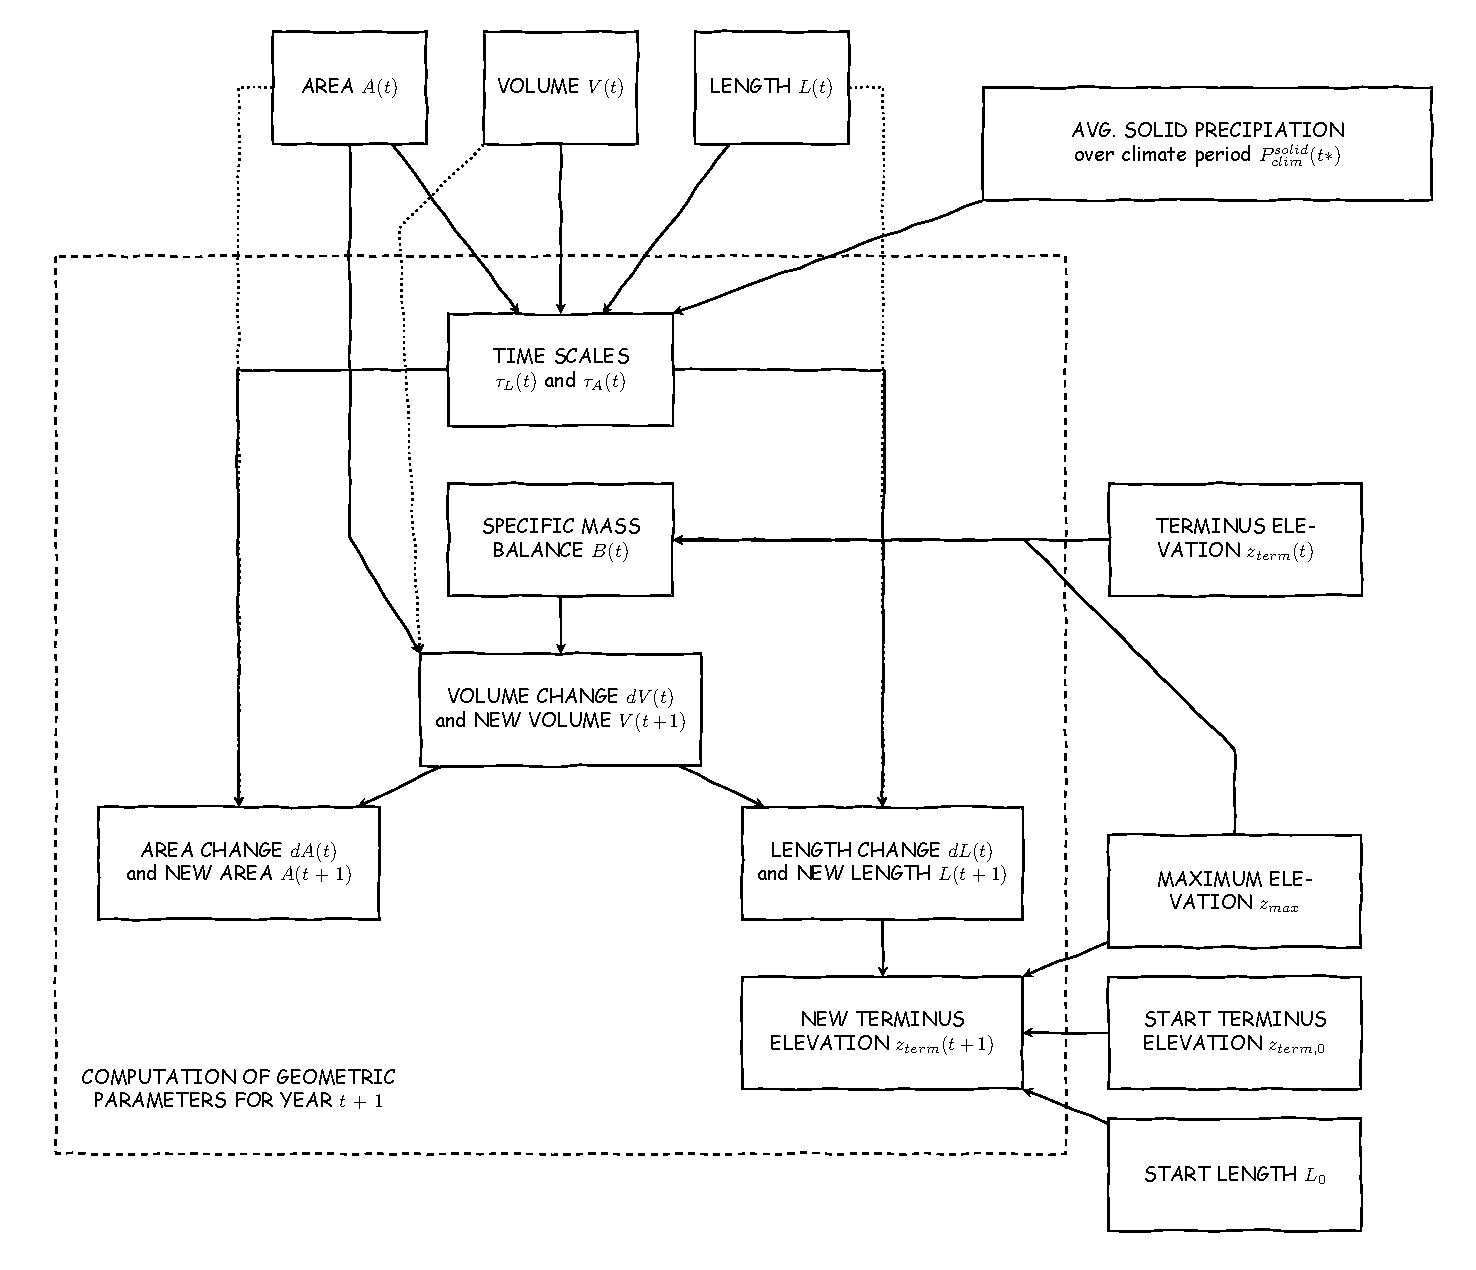
\includegraphics[width=\textwidth]{../flowchart/iterations/scaling.pdf}
            \caption{Schematic of the glacier evolution model's time stepping.}
            \label{fig:iteration-scheme}
        \end{figure}
    
    % subsection glacier_evolution_model (end)

% section general_concepts (end)

% ==== SECTION 2 ===============================================================
\section{Implementation} % (fold)
\label{sec:implementation}

    The \vas{} model is implemented in \href{https://www.python.org/}{Python 3}, following the code structure of the OGGM \citep{Maussion2019}. This compatibility is imperative, since the \vas{} model is no standalone project and relies on the OGGM for data downloads, preprocessing, post processing, and much more. The mass balance models and the glacier evolution model are implemented as classes with their respective methods. Functions outside these classes can be characterized either as entity tasks, which are applied on individual glaciers, or as global tasks, which run on a population of glaciers that need to share information between each other (mostly for calibration and validation). The entire code can be found on GitHub \url{https://github.com/OGGM/oggm-vas}, the following section can be seen as documentation.

    \subsection{Mass balance models} % (fold)
    \label{sub:mass_balance_models_implementation}

        Following the OGGM, the mass balance models are implemented as classes. The \lstinline`VAScalingMassBalance` model handles past or future climate data, while the \lstinline`ConstantVASMassBalance` model and the \lstinline`RandomVASMassBalance` model simulate a constant climate with and without inter-annual variability, respectively.

        \subsubsection{Volume/area scaling mass balance model} % (fold)
        \label{ssub:volume_area_scaling_mass_balance_model_implementation}

            The \lstinline`VAScalingMassBalance` model is the implementation of the original mass balance model by \citet{Marzeion2012b}. The model computes the mass balance of a glacier using historic or projected climate data provided by the climate input file. The general concept is fairly similar to the \lstinline`oggm.core.massbalance.PastMassBalance` model. The main difference is, that the \vas{} mass balance model returns only one average value of glacier-wide mass balance, instead of point mass balance values for the different elevation bands.

            The mass balance model is initialized for a single glacier, denoted by the OGGM specific glacier directory \lstinline`gdir`. Per default, the model will use the calibrated mass balance parameters \mustar{} and \bias{} and read temperature and precipitation records from the preprocessed climate file \lstinline`climate_historical`. An alternative climate file can be used, by supplying either the filename and/or it's suffix via the parameters \lstinline`filename` and \lstinline`input_filesuffix`, respectively. It is possible to specify the start year and end year of the climate period (\lstinline`ys` and \lstinline`ye`), if not all available data should be used. The parameter \lstinline`repeat` controls whether the climate period given by \lstinline`[ys, ye]` should be repeated indefinitely in a circular way.

            The \vas{} mass balance model inherits the following methods from the \lstinline`oggm.core.massbalance.MassBalanceModel` super class:
            \begin{itemize}
                \item \lstinline`get_annual_climate()` and \lstinline`get_monthly_climate()` compute and return the mass balance relevant climate information, i.e. positive air temperature at the terminus elevation in [\si{\celsius}] and solid precipitation amount in [\si{\kg\per\square\m}], for the given year and month/year combination, respectively.
                \item \lstinline`get_annual_mb()` and \lstinline`get_monthly_mb()` compute and return the glacier wide average mass balance in [\si{\m\per\s}], for the given year and month/year combination, respectively. A possible mass balance residual \bias{} is applied.
                \item \lstinline`get_specific_mb()` and \lstinline`get_monthly_specific_mb()` compute and return the glacier-wide average specific mass balance in [\si{mm w.e.\per yr}], for the given year and month/year combination, respectively. A possible mass balance residual \bias{} is applied.
            \end{itemize}
            All methods need the glacier terminus elevation \lstinline`min_hgt` and the maximal glacier surface elevation \lstinline`max_hgt` as input parameters. The date is supplied via the \lstinline`year` parameter, using the hydrological float year convention. Given that the scaling mass balance model computes the glacier-wide average mass balance, it is not possible to estimate the equilibrium line altitude. Hence, the the method \lstinline`get_ela()` is not implemented, in contrast to the \lstinline`PastMassBalance` model.
        
        % subsubsection volume_area_scaling_mass_balance_model_implementation (end)

        \subsubsection{Constant climate scenario} % (fold)
        \label{ssub:constant_climate_scenario_implementation}
            The \lstinline`ConstantVASMassBalance` model simulates a constant climate based on the observations averaged over a 31-year period centered on a given year \lstinline`y0`. Hence, the specific mass balance does not change from year to year. The task \lstinline`run_constant_climate(gdir, ...)` initializes a \lstinline`ConstantMassBalance` for the given glacier \lstinline`gdir` and runs for a given number of years \lstinline`nyears`. The task takes an additional temperature bias as parameters \lstinline`temp_bias`, to alter the observed climate records.

            The same idea of a constant climate is used during the mass balance calibration, solving the mass balance equation (Equation~\ref{eq:mass-balance}) for the temperature sensitivity \mustar. So per definition, \mustar{} is the temperature sensitivity to keep the glacier in equilibrium over the 31-year climate period centered around the \textit{equilibrium year} \tstar{}, while neglecting a potential mass balance residual \bias. Consequentially, a \lstinline`ConstantMassBalance` model with \lstinline`y0` = \tstar{} and \bias{} = 0 keeps the glacier in equilibrium.
        
        % subsubsection constant_climate_scenario_implementation (end)

        \subsubsection{Random climate scenario} % (fold)
        \label{ssub:random_climate_scenario_implementation}

            Similar to the \lstinline`ConstantVASMassBalance` model, the \lstinline`RandomVASMassBalance` model is based on a 31-year period centered on a given year \lstinline`y0`. However, the mass balance years are randomly shuffled within that period. More precisely, for each simulated year the model computes the specific mass balance using temperature and precipitation records from a randomly selected year within the given period. Hence, the model runs on a synthetic random climate scenario based on actual observations. A seed \lstinline`seed` for the random generator can be supplied as parameter, to allow for reproducibility. Additionally, it is possible to choose between draws with and without replacement via the \lstinline`unique_sample` parameter.

            The task \lstinline`run_random_climate(gdir, ...)` works analogously to the task \lstinline`run_constant_climate(gdir, ...)`, using an instance of \lstinline`RandomMassBalance` model instead of the \lstinline`ConstantMassBalance` model. Hence, using the climatological period centered around \lstinline`y0` = \tstar, the model glacier should stay in an equilibrium state while underlying minor fluctuations. Supplying a positive or negative temperature bias will result in a retreating or advancing model glacier, respectively, before reaching a new equilibrium after some years.
        
        % subsubsection random_climate_scenario_implementation (end)
    
    % subsection mass_balance_models_implementation (end)

    \subsection{Glacier evolution model} % (fold)
    \label{sub:glacier_evolution_model_implementation}

        The \lstinline`oggm-vas.VAScalingModel` is the implementation of the above describe glacier evolution model (see Section~\ref{sub:glacier_evolution_model}, cp. \citet{Marzeion2012b}) into the OGGM framework.

        An instance of the \lstinline`oggm-vas.VAScalingModel` class is initialized with the initial area \lstinline`area_m2_0`, the initial glacier terminus elevation \lstinline`min_hgt` and maximum glacier surface elevation \lstinline`max_hgt` and an instance of a mass balance model. Additionally, the start year of the simulation \lstinline`year_0` must be defined. Those initial values are stored as instance variables, since they are needed for later computations. Other than that, the \lstinline`oggm-vas.VAScalingModel` object stores all model parameters as instance variables for the year it is in. This includes glacier geometries ($V$, $A$, $L$, $z_\text{min}$, $z_\text{max}$) and their changes ($\Delta V$, $\Delta A$, $\Delta L$), time scales ($\tau_A$, $\tau_L$), the mass balance model and the specific mass balance $B$, but also constants like the scaling parameters ($c_A$, $\gamma$, $c_L$, $q$) and ice density $\rho_\text{ice}$.

        To advance the glacier model, there are three different methods. The \lstinline`step()` method advances the model by one year, following the above described steps (see Section~\ref{sub:glacier_evolution_model}). The method \lstinline`run_until(year_end)` runs the model until the specified year and returns the geometric glacier parameters at the end of the model evolution (year, length, area, volume, terminus elevation and specific mass balance). Thereby, the model starts from whatever year it currently is in. It is possible to start the model run from \lstinline`year_0` with the flag \lstinline`reset`. The method \lstinline`run_until_and_store()` works analogous to the previous one, with the difference that all parameters are stored for each time step (i.e., for each year). The resulting data set is returned and possibly stored to file, if a file path is give. The method \lstinline`run_until_equilibrium()` tries to run the glacier model until an equilibrium state is reached. The model runs for a fixed number of iterations \lstinline`max_ite`, the total elapsed time changes with the chosen time step \lstinline`ystep`. The iteration breaks, either if the glacier volume is below \SI{1}{\cubic\meter} or an equilibrium is reached. An equilibrium state is reached, if the volume change rate $|V(t) - V(t+\Delta t)|/V(t)$ falls below a given value \lstinline`rate`. Therefore, the method should only be used with a \hyperref[ssub:constant_climate_scenario_implementation]{constant climate scenario} (see Section~\ref{sub:mass_balance_models_implementation}).
    
    % subsection glacier_evolution_model_implementation (end)

% section implementation (end)


% ==== SECTION 3 ===============================================================
\section{Experimental setup} % (fold)
\label{sec:experimental_setup}
    
    % intro
    Implementing the \vas{} model is all good and well, but how does it compare to the flowline model?!
    While successfully passing the unit tests is a necessity---or at least good programming practice---unit tests are only testing for coding errors and not for the physicality of results. Nor do they answer the main research question: ``What information is gained from the use of a physical based flowline model?'' The following experiments run the newly implemented \vas{} model in a variety of setting and compare it to the flowline model. The focus is on the intrinsic model behavior and its comparison to the flowline model, not on absolute ice volume estimations.

    The experiments start on the smallest scale possible, namely with a single glacier. This first test case is intended to provide a feeling for the model and set the stage for the following experiments. Qualitative conclusions are drawn from time series of glacier geometries in response to different equilibrium climates. Some more quantitative results are obtained from an analysis of the autocorrelation function and the power spectral density of length change signals under a white noise climate, inspired by \citep{Roe2014}. Both analyses can only be performed on the signal of a single glacier, since mirroring oscillation of different glaciers could cancel each other out. To avoid a N-of-1 experiment, six different Alpine glaciers are investigated during this step. 
    However, scaling relations should not be applied to single glaciers. \Vas{} should only be applied to a collection of glaciers \citep{Bahr2015}. Hence, the next experiment runs the model for all glaciers in the European Alps. This first regional run looks at the evolution of aggregate ice volume for different equilibrium climate scenarios, in analogy to the single glacier test case.
    Any differences between the \vas{} model and the flowline model which emerge during these first experiments are most likely caused by the parameters defining the scaling relations. The response time scaling relation depends on the relaxation time scales for length and area, the volume/length and \vas{} relations depend on their respective scaling constants and scaling exponents. A sensitivity analysis of all those parameters is performed on a single glacier and on the collective Alpine glaciers.
    As a final experiment, the \vas{} model is used to estimate the potential ice melt of all Alpine glaciers during the coming one-hundred years. This is done by using todays climate in combination with different positive temperature biases, to simulate different warming climate scenarios.

    All the aforementioned experiments can be classified as equilibrium experiments. As most things in nature, glaciers strive toward a state of equilibrium. Such an equilibrium is reached eventually, by the glacier's adjusting of its geometry in reaction to changes in the climatic conditions. Analyzing the behavior of a glacier model subjected to a step change in climate can be used to get insights into the dynamics of the numerical model. The OGGM provides two convenient climate scenarios (or rather mass balance models) for such equilibrium experiment: the \lstinline`ConstantMassBalance` model and the \lstinline`RandomMassBalance` model. The implementation and workings of both mass balance models are described in Section~\ref{sub:mass_balance_models_implementation} (see \hyperref[ssub:constant_climate_scenario_implementation]{constant} and \hyperref[ssub:random_climate_scenario_implementation]{random} climate scenario).
    The hereafter detailed experiments use the HISTALP dataset \citep{Auer2007} as climate input data, with the corresponding hyper parameters (see Section~\ref{sub:temperature_index_model} for details).
    This obviously limits the suitable glaciers to the ones inside the HISTALP domain, i.e. the Alps. The Randolph Glacier Inventory (RGI, version 6.x) \citep{RGI2017,Pfeffer2014} lists 3892 glaciers for the region 11 subregion 01, which corresponds to the HISTALP domain.

    The following paragraph briefly lists the preprocessing tasks needed for the equilibrium runs. For a detailed description of the OGGM workflow see \citet{Maussion2019} and the \href{https://docs.oggm.org}{OGGM documentation}.
    \begin{description}[noitemsep]
        \item[GIS tasks:] using the NASADEM (\citet{NASADEM2020}, an updated version of the Shuttle Radar Topography Mission (\href{http://srtm.csi.cgiar.org/}{SRTM}), \citet{Jarvis2008})) as digital elevation model (DEM) and the RGI glacier outlines to compute a local grid, compute a glacier mask, compute centerlines and corresponding catchment areas;
        \item[climate tasks:] extract the HISTALP time series for the grid point nearest to the glacier and write it in the \lstinline`climate_historical.nc` file;
        \item[mass balance calibration:] computing the glacier specific mass balance parameters \tstar{}, \mustar{} and \bias{};
        \item[inversion tasks:] running the ice thickness inversion to estimate the bed topography (needed only for the flowline model);
    \end{description}

    The actual model runs are invoked via the \lstinline`run_constant_climate` and \lstinline`run_random_climate` tasks (see Section~\ref{sub:mass_balance_models_implementation} for implementation details). The used settings depend on the intended experiment and are detailed in the following sections.

    \subsection{Single glacier test case} % (fold)
    \label{sub:single_glacier_test_case_setup}

        The first qualitative look at the performance of the \vas{} model uses the Hintereisferner (RGI60-11.00897) as a test case. This test case is intended to get a feel for the model and set the stage for the following experiments, by comparing two evolution models and the two mass balance models.
        It has to be noted, that applying \vas{} to a single glacier gives only an order of magnitude estimate. The scaling constant $c$ is a globally averaged value, and the relative error in scaling constant is directly proportional to the error in estimated ice volume \citep{Bahr2015}. However, a qualitative comparison between the \vas{} model and the flowline model is more practicable and meaningful for a single glacier. The model's sensitivity to its scaling parameters is investigated in Section~\ref{sec:sensitivity_experiments_results}

        % Mass balance calibration and mass balance models using the same tstar
        For this first experiment, both evolution models run with the \lstinline`ConstantMassBalance` model and the \lstinline`RandomMassBalance` model, for 1000 years each. Both mass balance models emulate an equilibrium climate to keep the glacier in its initial equilibrium state. Therefore, the mass balance models must be initialized with the climatic period centered around the equilibrium year, i.e., \lstinline`y0` = \tstar{}. As explained above, the mass balance calibration depends among other parameters on \tstar{} (Section~\ref{sub:temperature_index_model}, see \hyperref[ssub:mb_calib]{Calibration of the mass balance parameters}). Hence, to run both evolution models with the identical climatic forcing, \tstar{} must be equal for both. This is done by using the same \tstar{} reference table (\lstinline`oggm_ref_tstars_rgi6_histalp.csv`, corresponding to the flowline model) to compute the temperature sensitivity \mustar{} for both models . Additionally, the mass balance residual must be omitted during the model run ($\beta^*$ = 0, as by the definition of \mustar{}, see Section~\ref{sub:temperature_index_model}). Each mass balance model runs three different climate scenarios defined by respective the temperature bias of \SI{0}{\celsius}, \SI{-0.5}{\celsius} and \SI{+0.5}{\celsius}. These results in a \emph{equilibrium run}, a run with \emph{positive mass balance perturbation} and a run with \emph{negative mass balance perturbation}, respectively.
    
    % subsection single_glacier_test_case_setup (end)

    \subsection{Autocorrelation function and Power spectral density} % (fold)
    \label{sub:autocorrelation_and_power_spectral_density_setup}

        The correlation is a measure for the linear dependency between two (random) variables. A positive correlation coefficient close to +1 indicates a strong direct relationship between the two variables, a negative correlation coefficient close to -1 indicates a strong indirect relationship, while a correlation coefficient around zero indicates that the variables are independent. The autocorrelation function (ACF) computes the correlation coefficient between a signal and a lagged copy of itself, as a function of lag time $k$. The lagged copy of a signal simply refers to the signal shifted by the lag time $k$. The intuition behind the ACF is the relation between past and present values of a signal. It is used find possible periodicities hidden in noisy signals and gives an estimate on how strong neighboring data points influence each other. A high autocorrelation at lag time $k$ indicates that data points at time $t$ and $t+k$ have similar values. The ACF at lag time $k=0$ is obviously one, since any signal correlates to \SI{100}{\percent} with itself. The partial autocorrelation function (PACF) measures only the direct influence of values with lag time $k$, eliminating the effects of all shorter lag times \citep{BoxJenkins2015}.

        On of the simples models to describe a stationary random time series is an autoregressive-moving-average (ARMA) model. It predicts future values of a random variable, based on a linear combination of past values and past error terms of said variable. The number of included lag terms is defined by the order $p$ of the autoregressive term and the order $q$ of the moving-average term. The number of statistically significant non-zero terms of the ACF and PACF can be used to estimate the order of an ARMA($p$,$q$) model, respectively \citep{BoxJenkins2015}. The linear three stage model by \citet{Roe2014} is an ARMA(3,3) model. While the goal of this work is not to define an ARMA glacier model, a brief analysis is provided in an attempt to quantify the autocorrelation.
        
        The power spectral density (PSD) is the Fourier transform of the ACF. A Fourier transformation decomposes a signal into a spectrum of frequencies, or much rather into a collection of frequency bins for the discrete Fourier transformation (DFT) used hereafter. Hence, the PSD is as function of frequency. The signal's power describes its energy per unit time. Thereby, the power is of unit \si{[X^2]} if the signal's unit is \si{[X]}, and must not be actual physical power of unit \si{[\watt]}. The power density is the power normalized with the frequency bin width, hence the power density has the unit \si{[X^2/\hertz]} if the frequency is measured in \si{[\hertz]}. The PSD is used to find dominant frequencies in noisy signals.

        The ACF, PACF and PSD are computed for the glacier length signal, in analogy to \citep{Roe2014}. To avoid N-of-1 experiment, the behavior of the \vas{} model is compared to the flowline model for the following six Alpine glaciers:
        \begin{itemize}
            \item Hintereisferner (RGI60-11.00897), Ötztal Alps, Austria
            \item Pasterze (RGI60-11.00106), Hohe Tauern, Austria
            \item Mer de Glace (RGI60-11.03643), Mont Blanc massif, France
            \item Glacier d'Argentière (RGI60-11.03638), Mont Blanc massif, France
            \item Großer Aletschgletscher (RGI60-11.01450), Bernese Alps, Switzerland
            \item Rhonegletscher (RGI60-11.01238), Urner Alps, Switzerland
        \end{itemize}
        These glaciers are selected because of their size and notoriety. However, the choice is somewhat arbitrary and most other glaciers would do the trick. All glaciers are subjected to different white noise climate conditions for 23\ 000 years. The remaining settings are analogous to the single glacier test case. The \lstinline`RandomMassBalance` model is initialized around the respective equilibrium year for each glacier (\lstinline`y0` = \tstar), whereby both evolution model use the same \tstar{} reference table (as before). The mass balance residual is omitted ($\beta^* = 0$). The input climate shows no autocorrelation and a constant PSD curve, and can therefore be classified as white noise with non-zero mean.
        To increase the amount of available data, each glacier is again subjected to three different climate scenarios, specified by a temperature bias of \SI{-0.5}{\celsius}, \SI{0}{\celsius} and \SI{+0.5}{\celsius}. The initial 3000 years during which the glaciers adjust to the changed climate are clipped, which leaves three different sizes of the same glacier, each in equilibrium.

        An ARMA model can only be applied to stationary time series. Stationarity is given if the mean and the variance are time independent and the signal shows no seasonality (for a formal definition see, e.g., \citet{BoxJenkins2015}). The stationarity of the glacier length signals could easily be determined manually. However, the formally more correct Augmented Dickey--Fuller test (\href{https://www.statsmodels.org/devel/generated/statsmodels.tsa.stattools.adfuller.html}{\lstinline`statsmodels.tsa.stattools.adfuller`}, \citet{Cheung1995-ADFuller}) is used to test for stationary. It results in $p$-values far below \SI{1}{\percent} for all signals. Hence, all signals can be considered as stationary.

        The ACF is computed using the python function \href{https://www.statsmodels.org/devel/generated/statsmodels.tsa.stattools.acf.html}{\lstinline`statsmodels.tsa.stattools.acf`} via a fast Fourier transform. The PSD is estimated using Welch's method. Welch's method reduces the variance in estimated power density. This is done by time-averaging at the cost of frequency resolution \citep[e.g.,][]{Welch1967, Proakis2007}. The remaining 20\ 000 data points (starting from year 3000) are divided into nineteen time windows with a window size of 2000  and a \SI{50}{\percent} overlap. The windows are tapered using the Hann function. For details about additional parameters see the default values of the python function \href{https://docs.scipy.org/doc/scipy/reference/generated/scipy.signal.welch.html}{\lstinline`scipy.signal.welch`}, which is used for the PSD computation.
    
    % subsection autocorrelation_fand_power_spectral_density_setup (end)

    \subsection{Regional runs with all Alpine glaciers} % (fold)
    \label{sub:regional_runs_with_all_alpine_glaciers_setup}
        \Vas{} applied to single glaciers gives only an order of magnitude estimation, since the scaling constant $c$ is a globally averaged value. A potential relative error in $c$ will be directly transfered to any volume estimation. Hence, \vas{} should only be applied to collections of glaciers \citep{Bahr2015}. 
        The first regional simulation runs with all Alpine glaciers. The experimental setup is analogous to the single glacier test case, again comparing the \vas{} model to the flowline model, with some minor modifications. To best reflect the regional glacial evolution, the default OGGM \hyperref[ssub:mb_calib]{mass balance calibration} is used (see Section~\ref{sub:temperature_index_model}). This means, each evolution model uses its own \tstar{} reference table (which may result in different \tstar{} for the same glacier depending on the evolution model). The mass balance residual is still omitted ($\beta^* = 0$), since this experiment is again intended towards the investigation of model behavior rather than absolute real-world values.
        Both evolution models run with the \lstinline`ConstantMassBalance` model and the \lstinline`RandomMassBalance` model, for 1000 years each. The mass balance models are initialized with \lstinline`y0` = \tstar{} and run with the same three different temperature biases as before (\SI{0}{\celsius}, \SI{-0.5}{\celsius}, \SI{+0.5}{\celsius}).
    
    % subsection regional_runs_with_all_alpine_glaciers_setup (end)

    \subsection{Sensitivity experiments} % (fold)
    \label{sub:sensitivity_experiments_setup}
        % introduction
        Before moving to the final experiments, the projection of future ice mass loss for all Alpine glaciers, it is necessary to determine the model's sensitivities. The following sensitivity analysis investigates the effects of the model-internal time scales and the scaling parameters on the model behavior. Both parameter sets are specific to the scaling model, since they determine the response time scaling as well as the volume/length and \vas{}. For consistency, the sensitivity experiments are performed on Hintereisferner (RGI60-11.00897) as a single glacier test case and on all Alpine glaciers inside the HISTALP domain. For simplicity, only the \lstinline`ConstantMassBalance` model with a temperature bias of \SI{+0.5}{\celsius} is used for all runs.

        % Time scales
        The scaling model estimates glacial evolution via the implemented response time scaling. Response time scaling adjusts the yearly changes in length and area, in relation to the total possible changes, using the model-internal response time scales for length and area, $\tau_L$ and  $\tau_A$, respectively.
        The estimate for the model-internal time scales loosely follows \citet{Johannesson1989} (see Section~\ref{sub:glacier_evolution_model} and \ref{sub:glacier_evolution_model_implementation} for details). However, the model-internal time scales are good possible tuning parameters. The sensitivity experiments compare the model output for different time scales, modified by a linear factor $\tau_\text{sens.} = f \cdot \tau$. Hereby, the factor $f$ is only applied to $\tau_L$, since $\tau_A$ is a just linear function of $\tau_L$. Starting from the default value ($f=1$) as baseline, the effects of halved ($f=0.5$) and doubled ($f=2$) model-internal time scales are investigated.

        % Scaling parameters
        The other obvious choice for tuning parameters are the scaling exponents and scaling constants. The scaling constants for volume/length and \vas{}, $c_L$ and $c_A$, respectively, can be seen as random variables. The randomness stems from the statistically similar, but not identical, dimensionless parameters for length, area and volume  varying from glacier to glacier. Thanks to the law of large numbers, the global scaling constants $c_L = \SI{0.0180}{\kilo\meter^{3-q}}$ and $c_A = \SI{0.0340}{\kilo\meter^{3-2\gamma}}$ are a reasonable choice for a global ice volume estimation \citep{Bahr2015}. However, those parameters may be a bad fit for certain regions and therefore need calibration.
        While the scaling constants are not constant, the scaling exponents are. The \vas{} exponent was first derived as the slope of the linear regression of volume and area observations in log-log space \citep[e.g.,][]{Chen1990}. \citet{Bahr1997b} found that their values are fixed by the underlying physics and depend only on a single set of closure conditions. The closure conditions are in turn tightly bound by observations. Different common closures lead to the same results. Hence, it is strongly advised to use the global values of $q = 2.2$ and $\gamma = 1.375$  for the volume/length and \vas{}. Furthermore, even if different closure conditions could be justified, the area scaling exponent is bound $1.1\dot{6} \leq \gamma \leq 1.5$ by simple geometric reasoning \citep[Section 8.2]{Bahr2015}. 

        As for the time scale sensitivity experiments, the global values of the scaling exponents serve as baseline. The next run uses custom scaling constant derived from a linear regression in log-log space but with a fixed slope corresponding to the global scaling exponents. The last run uses full custom scaling constants and exponents, again derived from a linear regression in log-log space. For reasons of simplicity, data points of volume, area and length are taken from the OGGM flowline model glaciers and not from observations. The inversion volume serves as glacier volume, the RGI area as surface area and the longest centerline as glacier length.
        
        Since a linear regression can not be computed from a single data point, the Hintereisferner test case differentiates only between global and custom scaling constants (obtained by solving the scaling relations for $c$) while using the global default scaling exponents in both cases. The following two sets of scaling parameters are used:
        \begin{enumerate}[label=(\alph*)]
            \item global (default) values of $c_L = \SI{4.551}{\meter^{3-q}}$, $q = 2.2$ for volume/length scaling and $c_A = \SI{0.191}{\meter^{3-2\gamma}}$, $\gamma = 1.375$ for \vas{}
            \item custom scaling constants $c_L = \SI{1.555}{\meter^{3-q}}$ and $c_A = \SI{0.252}{\meter^{3-2\gamma}}$ with the global and physically based scaling exponents $q = 2.2$ and $\gamma = 1.375$
        \end{enumerate}
        For comparability, the sensitivity runs on Hintereisferner (RGI60-11.00897) are setup exactly the same as the test case (see Section~\ref{sub:single_glacier_test_case_setup}). This means a fixed \textit{equilibrium year} $t^{*} = 1927$ and no mass balance residual during the run. The regional Alpine runs are setup as before (see Section~\ref{sub:regional_runs_with_all_alpine_glaciers_setup}) and use the following three sets of scaling parameters:
        \begin{enumerate}[label=(\alph*)]
            \item global (default) values of $c_L = \SI{4.551}{\meter^{3-q}}$, $q = 2.2$ for volume/length scaling and $c_A = \SI{0.191}{\meter^{3-2\gamma}}$, $\gamma = 1.375$ for \vas{}
            \item custom scaling constants $c_L = \SI{1.805}{\meter^{3-q}}$ and $c_A = \SI{0.250}{\meter^{3-2\gamma}}$ with the global and physically based scaling exponents $q = 2.2$ and $\gamma = 1.375$
            \item custom scaling constants and scaling exponents $c_L = \SI{0.244}{\meter^{3-q}}$, $q = 2.517$ for volume/length scaling and $c_A = \SI{0.117}{\meter^{3-2\gamma}}$, $\gamma = 1.441$ for \vas{}
        \end{enumerate}

        Disclaimer: As already mentioned, this work is focused on the model behavior much rather than an absolute ice volume estimation. While scaling constants and exponents based in observations would be preferable, the values of the custom scaling parameters are not as important for these sensitivity experiments, as long as the are different from the global values. In fact, the sensitivity experiment could easily be conducted with a set of fabricated exponents. For the same reason, it is also inconsequential that scaling exponents derived from a numerical model depend on the model's closure conditions \citep[Section 8.9]{Bahr2015}. This potential source for errors is acknowledged, but the flowline model is not tested for its closure conditions. While the custom scaling exponents lie within the range of physical sensible values, finding closure conditions supporting the computed values would go (far) beyond the scope of this work.

    % subsection sensitivity_experiments_setup (end)

    \subsection{Commitment runs} % (fold)
    \label{sub:commitment_runs_setup}
        One of the easiest ways of estimating future glacial evolution are so called \textit{commitment runs}.
        The term stems from the \textit{commitment} to a given climate, which is then held constant for the entire run. By this definition, all experiments detailed above can be classified as commitment runs. However, in this context, commitment runs refer to projections of future changes in ice mass. For example, applying the current climate to the current glacier geometries for the next, say, 100 years, would give a---naively optimistic---lower bound of the expected glacial retreat.

        While a climate scenario with year-to-year fluctuations is more realistic and a completely constant climate is not, the resulting changes in regional ice volume over a longer time period are comparable (see Section~\ref{sec:regional_runs_with_all_alpine_glaciers_results}). Therefore, the following experiments can be limited to the \lstinline`ConstantMassBalance` model without any loss of information. The \lstinline`ConstantMassBalance` model is initialized with todays climate. Todays climate is defined as the average over the most recent 31 years. For the HISTALP dataset this corresponds to the period from 1984 to 2014 with \lstinline`y0 = 1999`. Since we live in a period of global warming, additional positive temperature biases of \SI{0}{\celsius}, \SI{+0.5}{\celsius}, \SI{+1.0}{\celsius} and \SI{+2.0}{\celsius} are used. Besides using the default OGGM \hyperref[ssub:mb_calib]{mass balance calibration}, potential mass balance residuals \bias{} are applied to all glaciers, assuring the most physical outcome. The simulation starts with the RGI glacier geometries (from around 2003), without any spinup period. Thereby, the imbalance between current glaciers and current climate is not considered.
    
    % subsection commitment_runs_setup (end)

% section experimental_setup (end)